\documentclass[11pt,a4paper,oneside]{report}
\usepackage[T1]{fontenc}
\usepackage[utf8]{inputenc}
\usepackage{lmodern}
\usepackage[margin=25mm]{geometry}
\usepackage{microtype}
\usepackage{amsmath,amssymb}
\usepackage{graphicx,booktabs,tabularx,longtable,array}
\usepackage{xcolor,listings,enumitem}
\usepackage{xurl}
\usepackage[hidelinks]{hyperref}
\usepackage{bookmark}
\usepackage{titlesec}
\titlespacing*{\chapter}{0pt}{0pt}{20pt}
\definecolor{draftred}{HTML}{9A402D}
\definecolor{codebg}{HTML}{F3F5F7}
\newcommand{\todo}[1]{\par\smallskip\noindent\textcolor{draftred}{\textbf{To complete:} #1}\par\smallskip}
\newcommand{\code}[1]{\nolinkurl{#1}}
\setlength{\emergencystretch}{2em}
\newcommand{\placeholder}[2]{\begin{figure}[htbp]\centering\fbox{\parbox[c][24mm][c]{0.88\linewidth}{\centering #1}}\caption{#2}\end{figure}}
\lstset{basicstyle=\ttfamily\small,backgroundcolor=\color{codebg},breaklines=true,columns=fullflexible,keepspaces=true,showstringspaces=false,frame=single,rulecolor=\color{black!15},framesep=5pt}
\setlist{itemsep=3pt,topsep=5pt}
\setlength{\parskip}{5pt}
\setlength{\parindent}{0pt}
\setcounter{tocdepth}{1}
\title{Experimental Technical Notes\\[8pt]\Large Technical Handover}
\author{Zuchen Huang}
\date{3 November 2026}
\begin{document}
\maketitle
\chapter*{About this document}
\addcontentsline{toc}{chapter}{About this document}
This document collects technical details and practical guidance for ALLEGRO PCB evaluation. It describes how to reproduce the PCB measurements and interpret their results, including setup details and operating experience that are not captured in the analysis scripts. Its scope also includes simulations of the minimum and maximum energy deposits relevant to PCB evaluation; these will be documented in a separate chapter.

For questions, corrections or clarification, please contact Zuchen Huang at \href{mailto:zuchen.huang@cern.ch}{\nolinkurl{zuchen.huang@cern.ch}}.
\begingroup
\small
\setlength{\parskip}{0pt}
\tableofcontents
\endgroup
\chapter{PCB Testing}
\label{ch:pcb-testing}
\section{PCB under test}
\label{sec:pcb-overview}
The measurements described in this chapter characterise the cross-talk and capacitance of a PCB designed for the ALLEGRO barrel calorimeter (Figure~\ref{fig:pcb}). This note is based on cern PCB v2 and China PCB v1. For measurements of an endcap PCB or a different board layout, update the topology-dependent channel maps and geometry parameters in the analysis scripts before using them.

\subsection{Tower layouts}
The board contains 16 towers with different signal-routing layouts or structural features. Towers 1, 2, 15 and 16 explore different strip-layer sizes or positions; the other towers explore different signal-path matching and shielding arrangements. Refer to the PCB layout drawing for the detailed configuration of each tower.

Each tower has a 16-pin connector. With the connector at the top of the board, the connector channels are numbered from right to left, from 1 to 16. In the logical-trace (\code{logTrac}) layout, cell 1 is the cell farthest from the connector. The channel-to-cell mapping follows the cell order, starting with channel 1 for cell 1, with channel 8 skipped. For the optimal-trace layout, use the tower-specific mappings in \code{default_config.m}; the maps currently implemented in the toolkit are listed in Section~\ref{sec:tower-maps}.

Connector-channel numbering must be distinguished from the toolkit's acquisition-channel and display conventions described in Section~\ref{sec:channel-conventions}.
\todo{Add an annotated connector pinout showing how all 16 connector channels correspond to the 15 acquisition channels, including the role of channel 8 and the exact cell numbering after it is skipped. Identify the viewed side of the PCB so that right-to-left numbering is unambiguous.}

\subsection{Scope of the measurements}
The toolkit supports two measurements: a cross-talk matrix and a per-channel capacitance measurement. Each tower has 15 acquisition channels. A full cross-talk scan records all 225 injection/readout combinations. A capacitance scan records 15 waveforms with injection and readout routed to the same channel. Capacitance is obtained offline by comparing the fitted time constants with a separately acquired T0 reference.

The multiplexer selects channels within the connected tower. It does not change the physical tower connection. The operator must reconnect the apparatus and update the tower number between towers.
\todo{Record the board revision and add the PCB layout drawing with tower identifiers. Explain the construction and electrical meaning of the T0 reference.}

\begin{figure}[p]
    \centering
    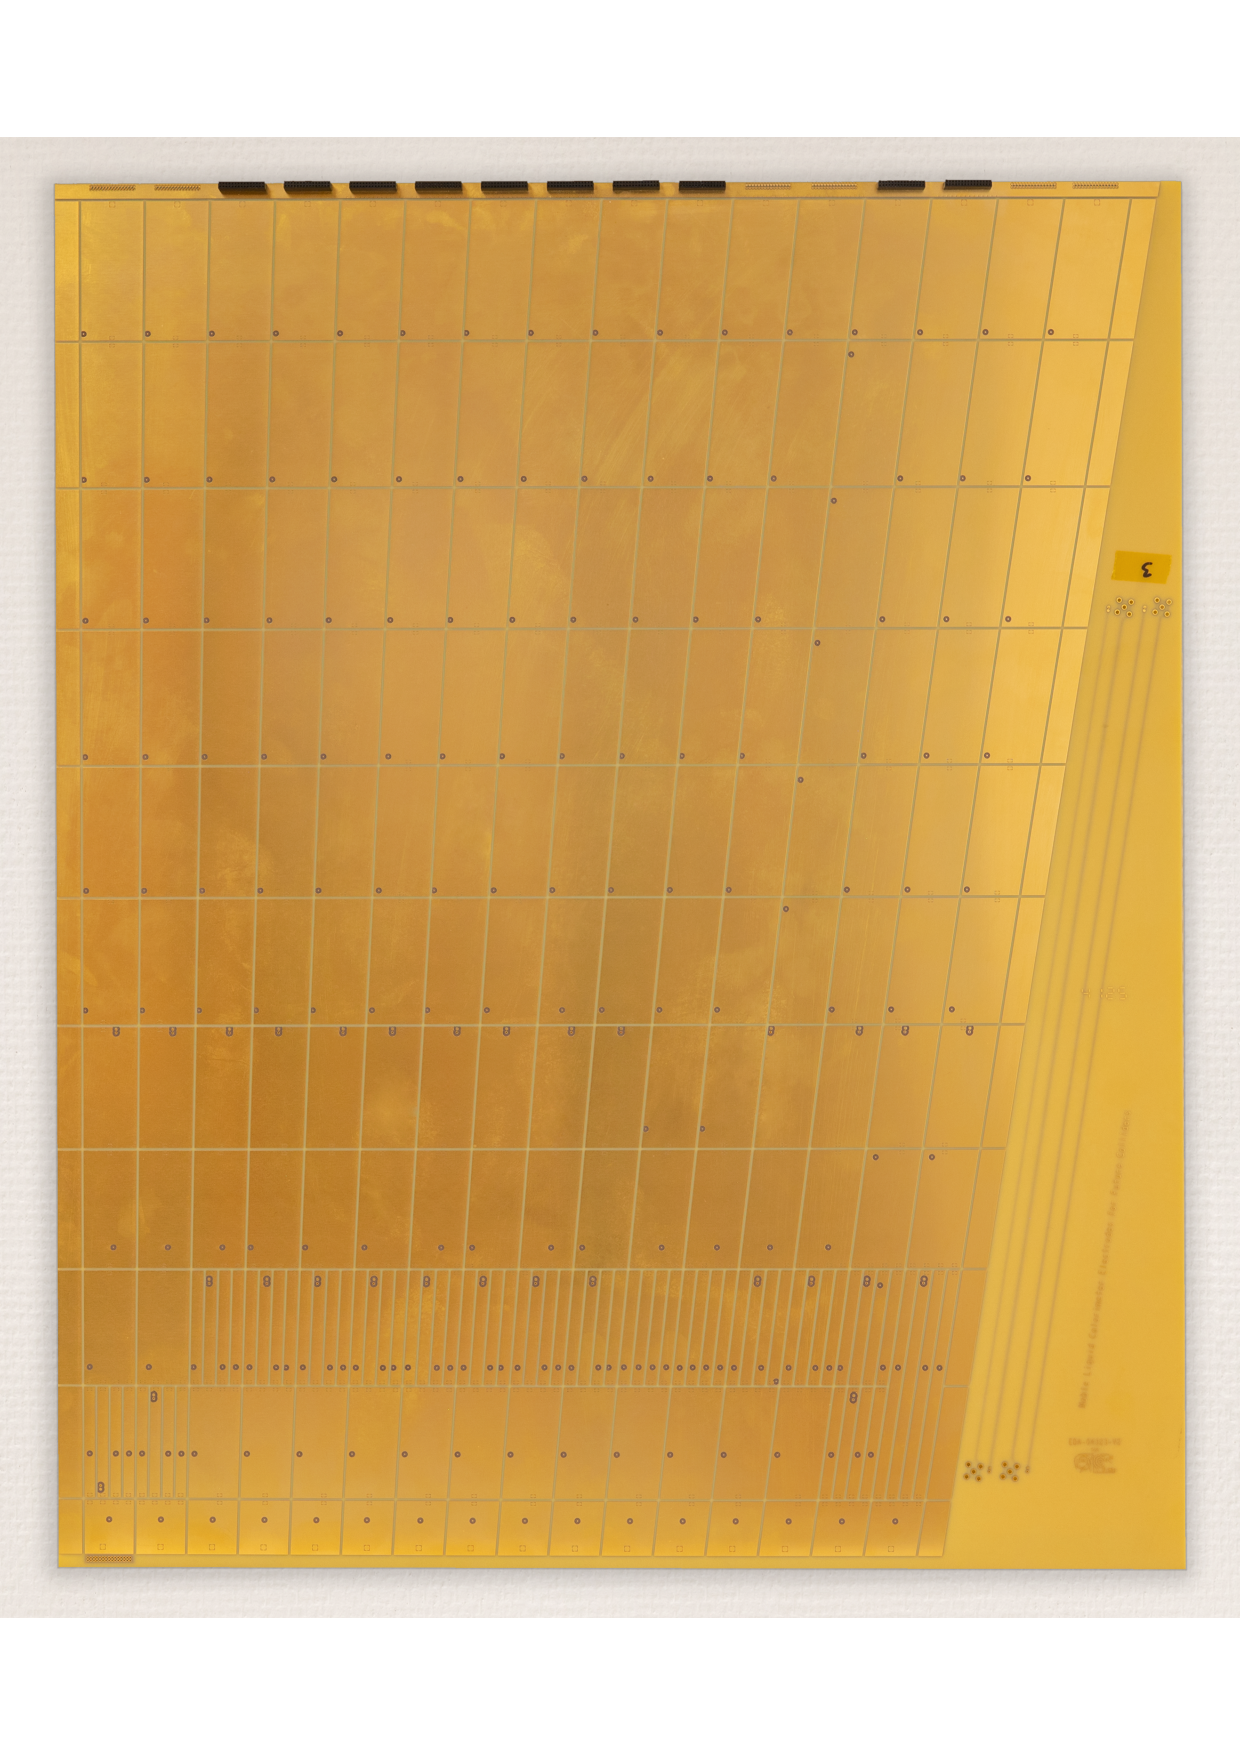
\includegraphics[width=\linewidth,height=0.82\textheight,keepaspectratio]{figures/PCB_ver2.pdf}
    \caption{ALLEGRO barrel calorimeter PCB with 16 towers. The connectors are along the upper edge in this view. Refer to the PCB layout drawing for tower identifiers and routing details.}
    \label{fig:pcb}
\end{figure}

\section{Measurement setup and conventions}
\label{sec:setup}
\subsection{Signal path and instrument roles}
The acquisition software assumes that oscilloscope CH1 carries the direct generator reference and CH2 carries the multiplexer readout. The scripts configure and read CH2 only. CH1 and the trigger are set on the instrument by the operator. The exact generator branching, loading and connector arrangement must be documented from the bench.
\placeholder{Insert an annotated wiring diagram and a photograph of the connected setup.}{Setup documentation to be added. Label generator output, reference branch, injection path, readout path, multiplexer connectors, tower orientation and scope inputs.}

\begin{tabularx}{\linewidth}{@{}lX@{}}
\toprule
Element & Role and information to record \\
\midrule
Signal generator & Excitation source; model, output mode, amplitude convention and load. \\
Multiplexer & Routes injection and readout channels; model, connector pinout and GPIB address. \\
Oscilloscope & Single-shot capture of CH2; model, firmware, input settings and trigger. \\
Windows PC & VISA communication and MATLAB acquisition. \\
Offline computer & MATLAB analysis and result export; may be separate from the acquisition PC. \\
\bottomrule
\end{tabularx}
\todo{Add instrument models and serial numbers, generator waveform/frequency/amplitude/offset, termination and probe settings, scope coupling and bandwidth, sample rate, record length, time window and trigger settings. Cross-talk and capacitance may need separate setup records.}

\subsection{Three channel-number conventions}
\label{sec:channel-conventions}
An \emph{acquisition channel} is the number 1--15 passed to the multiplexer. A \emph{display position} follows \code{cfg.displayOrder}; position 8 is omitted from the cross-talk heatmap after reordering. A \emph{study cell} follows the separate \code{cfg.studyCellToChannel} map. These conventions must be kept distinct when comparing a plotted cell with a physical connector.

The cross-talk scan's adjacent-pair preset is selected by
\[
 |i-j|=1,
\]
where $i$ and $j$ are acquisition-channel numbers. This condition alone does not establish physical adjacency on the PCB.
\todo{Complete the connector-to-acquisition-channel map introduced in Section~\ref{sec:pcb-overview}, explain why display position 8 is omitted, and identify physical neighbours for each board layout.}

\section{Installation and communication checks}
\label{sec:installation}
\subsection{Acquisition environment}
The historical installation note describes Windows 10 with a Keysight 82357B USB--GPIB adapter. It uses Keysight IO Libraries Suite, installing the prerequisite package before the main package when supplied separately. The optional NI route uses NI Package Manager to install NI-VISA and NI System Configuration, including Measurement \& Automation Explorer (MAX).

Treat this as a record of the previous setup. Select installer versions compatible with the actual PC and adapter, and record the working combination rather than assuming that a newer release reproduces it. Useful vendor entry points are \href{https://www.keysight.com/us/en/lib/software-detail/computer-software/io-libraries-suite-downloads-2175637.html}{Keysight IO Libraries Suite} and \href{https://www.ni.com/en/support/downloads/software-products/download.package-manager.html}{NI Package Manager}. These links were carried over from the installation note and were not checked for current instructions.
\todo{Record Windows, MATLAB, VISA provider and driver versions from the working instrument PC. Confirm whether NI software is needed and document any coexistence settings. The old note's MATLAB platform-support statement needs current verification.}

\subsection{Verify communication before running a scan}
Connect the instruments and check that they appear in Keysight Connection Expert (or the installed equivalent). Use the instrument's interactive I/O facility to query its identity with \code{*IDN?}, where supported. Confirm that the returned identity corresponds to the connected matrix or scope.

The old installation note demonstrates GPIB communication with an HP 6624A supply using \code{VSET 1 2} and \code{VOUT? 1}. These are supply-specific examples, not commands for the PCB multiplexer or oscilloscope.

In MATLAB, enumerate the available resources:
\begin{lstlisting}
resources = visadevlist;
disp(resources)
% Example only: replace with the resource reported on this PC.
scope = visadev('USB0::0x0AAD::0x01D6::105097::0::INSTR');
identity = strtrim(writeread(scope, '*IDN?'));
clear scope
\end{lstlisting}
Use the reported resource names in the acquisition entry scripts. Do not select an instrument by its row number in \code{visadevlist}: enumeration order can change. Close exploratory connections before handing the same resource to a script.

The current scripts contain example resources \code{GPIB0::7::INSTR} for the matrix and \code{USB0::0x0AAD::0x01D6::105097::0::INSTR} for the scope. Neither should be assumed to match another PC. The optional \code{matrixIdContains} and \code{scopeIdContains} settings can enforce expected identity text; empty strings disable those checks.

\subsection{MATLAB dependencies and path}
\begin{tabularx}{\linewidth}{@{}lX@{}}
\toprule
Task & Dependency \\
\midrule
Acquisition & Instrument Control Toolbox and working VISA connections. \\
Cross-talk shaping & Control System Toolbox. \\
Cross-talk study plots & Signal Processing Toolbox, in addition to shaping dependencies. \\
Capacitance waveform fitting & Optimization Toolbox. \\
\bottomrule
\end{tabularx}

Keep the five \code{run_*.m} scripts and the \code{+pcbtest} package together. Each entry script adds the toolkit root to the current MATLAB session without changing the saved path. For direct function calls:
\begin{lstlisting}
addpath('path/to/pcb_test_toolkit');
cfg = pcbtest.default_config(4);
\end{lstlisting}
\todo{Record the tested MATLAB release and toolbox versions. Confirm access to the toolkit repository or shared archive for the next operator.}

\section{Toolkit and data organisation}
\label{sec:toolkit}
\subsection{Entry points}
\begin{tabularx}{\linewidth}{@{}lX@{}}
\toprule
Script & Purpose \\
\midrule
\code{run_acquire_debug.m} & One injection/readout pair; saving disabled by default. \\
\code{run_acquire_xtalk.m} & One tower's complete $15\times15$ cross-talk scan. \\
\code{run_acquire_capacity.m} & One tower's 15 capacitance waveforms; also used for T0. \\
\code{run_offline_xtalk.m} & Cross-talk analysis for a list of towers. \\
\code{run_offline_capacity.m} & Capacitance analysis relative to T0. \\
\bottomrule
\end{tabularx}

\code{+pcbtest/default_config.m} defines shared settings and channel maps. Entry scripts override selected fields, so the settings at the top of the chosen script are part of the measurement configuration. For example, the current cross-talk script uses ranges 5, 0.3 and 0.1, whereas the shared defaults use 5, 0.15 and 0.08.

\subsection{Parameters to set for each campaign}
Before acquisition, check \code{tower}, \code{dataRoot}, \code{datasetLabel}, the two VISA resource names, CH2 settings and \code{skipExistingFiles}. Set identity checks where practical. For offline analysis, set \code{towers}, \code{dataDir}, \code{datasetLabel}, \code{outputLabel} and \code{towerSubfolders}. The cross-talk script also exposes \code{shapingTimes} and \code{studyCells}.

The current acquisition and offline cross-talk scripts both use \code{data/xtalk_run_001}. The README's acquisition example mentions \code{xtalk_run_003}; use the actual configured path. Prefer a fresh campaign directory when changing the setup.

\subsection{Raw waveform files}
A typical campaign is organised as follows:
\begin{lstlisting}
pcb_test_toolkit/
  +pcbtest/
  run_acquire_xtalk.m
  ...
  data/
    xtalk_run_001/T4/T4_xtalk_PCBCHINA_01-02.mat
    capacity_run_001/T0/T0_Capacity_PCBCHINA_1.mat
    capacity_run_001/T4/T4_Capacity_PCBCHINA_1.mat
  output/
    PCBCHINA/xtalk/T4/
    PCBCHINA/capacity/T4/
\end{lstlisting}
In a cross-talk filename, the first two-digit number is the injection channel and the second is the readout channel. Capacitance filenames use an unpadded channel number. Cross-talk files contain \code{t} in seconds and \code{data} in volts; capacitance files contain \code{t} and \code{data_read}. New acquisitions also save \code{metadata} with acquisition time, tower, channel information, instrument identities and the applied CH2 vertical settings.

The metadata is not a complete record of the bench: generator parameters, scope trigger, timebase, actual tower wiring and toolkit revision are not saved by these acquisition functions. Record them separately. Debug acquisition with \code{applyScopeSettings = false} saves no numerical front-panel vertical settings.

\subsection{Existing files and interrupted scans}
With \code{skipExistingFiles = true}, the script loads each existing waveform and checks its metadata against the selected channels, tower, readout scope channel, vertical settings and instrument identities. A mismatch stops the scan. Historical files without matching metadata cannot be resumed this way.

With \code{skipExistingFiles = false}, matching filenames are acquired again and overwritten. The current cross-talk entry script uses \code{false}; the capacitance script uses \code{true}. Metadata matching does not verify unsaved settings such as generator amplitude or trigger configuration. Resume only after confirming those independently.

The toolkit ignores the entire \code{output/} directory in Git. Keep raw data, configuration records and analysis outputs in the laboratory's chosen archive; a code checkout alone does not preserve the measurement.

\section{Practical procedure at the bench}
\label{sec:practical}
\subsection{Prepare the measurement}
\begin{enumerate}
\item Identify the board, tower and measurement type. Start a campaign record using Section~\ref{sec:record} and select a new data directory.
\item Connect the chosen tower. Double check if you connect only to one row of pins.
\item Set the generator, scope inputs, horizontal acquisition settings and trigger for the measurement. Confirm the direct generator reference on CH1.
\item Verify both VISA resources and their identities as described in Section~\ref{sec:installation}.
\end{enumerate}

\subsection{Inspect one pair before a scan}
Open \code{run_acquire_debug.m}. Set the tower, injection channel, readout channel and VISA resources. Use a diagonal pair first, then inspect an adjacent-number pair and another off-diagonal pair to assess the three cross-talk presets.

With \code{applyScopeSettings = true}, the script sends its position, range and offset to CH2. With \code{false}, it keeps the front-panel vertical settings. Its default is \code{true}; the current debug values are not automatically matched to the cross-talk presets. Set \code{saveWaveform = true} if the diagnostic waveform should be preserved.

Run the script. It starts immediately without a confirmation prompt, routes one pair, requests \code{SING}, waits for \code{*OPC?} to return \code{1}, waits the configured read delay and reads CH2. The matrix receives the cleanup command \code{C} on normal exit or error cleanup. The captured waveform remains available for inspection on the scope.

Check that the trigger is stable, the waveform is not clipped, and the time window contains the baseline and relevant response. For capacitance, check that the positive rising waveform and its approach to the plateau are captured. For cross-talk, inspect the small off-diagonal signals at their intended scales.
\placeholder{Insert diagonal, off-diagonal and capacitance waveform examples.}{Representative successful acquisitions, with timebase, vertical settings and channel pair recorded. Add examples of clipping and incorrect triggering for comparison.}
\todo{Add expected waveform polarity, approximate amplitudes and timescales, baseline/noise examples, and the laboratory's acceptance criteria. These cannot be inferred reliably from the software alone.}

\subsection{Acquire cross-talk}
\begin{enumerate}
\item In \code{run_acquire_xtalk.m}, set the connected tower, campaign directory and dataset label. Check all three CH2 presets and the overwrite/resume switch.
\item For an initial trial, use a separate data directory and change \code{cfg.channels = 1:2}. This creates four pair files. Inspect them before the full scan; the offline matrix analysis requires all 225 pairs and cannot analyse the trial alone.
\item Restore \code{cfg.channels = 1:15}, choose the full-run directory and run the script. Confirm the displayed tower by pressing Enter, or type \code{q} to stop.
\item Follow the saved-file messages. A full scan has 225 expected filenames. Check filename coverage and representative waveforms after completion; the count alone does not prove that the physical tower was correct.
\item To scan another tower, change the physical connection, update \code{tower}, verify the setup again and rerun the script.
\end{enumerate}
The current script uses a 0.5-second delay after confirmed acquisition and before waveform readout. The shared pre-acquisition settling default is zero. These are software settings, not a validated settling-time study.

\subsection{Acquire capacitance and T0}
\begin{enumerate}
\item Configure the capacitance excitation and scope settings. Use a square-wave frequency in the kHz range, with sufficient time for charging and discharging. Set the acquisition window to include a pre-rise baseline and the rising response approaching its plateau, ending before the next falling edge; the current fitter uses all samples after threshold crossing. Record the exact frequency and duty cycle. Connect T0 and set \code{tower = 0} in \code{run_acquire_capacity.m}.
\item Choose the capacitance campaign directory and dataset label. Check the CH2 range and the overwrite/resume switch. The shared position and offset are $-4$ and 0; the entry script's range is 2.
\item Run the script and confirm the T0 connection. It routes injection and readout to each channel in turn and saves 15 files.
\item Connect a measurement tower, update \code{tower}, and acquire its 15 files under the same campaign root and dataset label. Record any changes to the setup between T0 and the tower.
\end{enumerate}
The capacitance scan waits 2 seconds after routing/configuration and 1 second after confirmed acquisition before readout, using the current defaults. Fitting is performed offline.
\todo{Specify when T0 should be remeasured, how reference stability is checked, and how to handle a setup change during a campaign. Explain the physical reference subtraction.}

\subsection{Run offline analysis and archive}
Copy the raw campaign directory and the measurement record to the offline computer. For cross-talk, set \code{run_offline_xtalk.m} to the campaign root and tower list. The current shaping times are 20, 50 and 200 ns; setting \code{studyCells = []} skips the study plots. Keep \code{towerSubfolders = true} for the toolkit's directory layout.

For capacitance, point \code{run_offline_capacity.m} to the common directory containing T0 and the measurement towers. Exclude T0 from \code{towers}: it is loaded as the reference. Its fitted tau array is reused across towers during the script run. Choose a distinct \code{outputLabel} when retaining multiple analyses.

Review plots, numerical exports and warnings using Section~\ref{sec:analysis}. Archive the raw files, the exact edited entry scripts, toolkit revision, setup record, reference dataset and analysis outputs together.

\subsection{Troubleshooting guide}
The checks below are diagnostic starting points, not an established list of failure causes.
\begin{longtable}{@{}p{0.30\linewidth}p{0.65\linewidth}@{}}
\toprule
Observation & Check or next action \\
\midrule
\endhead
Instrument missing & Check physical connection and vendor discovery first; then check MATLAB's resource list and the selected VISA installation. \\
No acquisition completion & Inspect trigger source, level and whether a trigger is actually arriving. Record the instrument response and MATLAB error. \\
Unexpected or clipped waveform & Check the selected pair, physical routing, input settings, and the complete CH2 preset. Compare with a saved known-good trace. \\
Existing-file mismatch & Compare metadata and campaign settings. Use a new directory for a changed setup; overwriting replaces earlier measurements. \\
Cross-talk analysis stops & Check all 225 filenames, the dataset label and the reported malformed or mismatched-time-axis file. \\
Capacitance channel is NaN & Inspect both tower and T0 waveforms for that channel, threshold crossing, fit convergence and the acquisition window. \\
Plot disagrees with board label & Translate acquisition channel, display position and study cell through the appropriate maps. \\
\bottomrule
\end{longtable}
\todo{Add actual recurring bench problems and their confirmed fixes, preferably with example traces and instrument messages.}

\section{Analysis definitions and interpretation}
\label{sec:analysis}
\subsection{Cross-talk shaping and amplitudes}
Each waveform is baseline-corrected by subtracting the mean of its first 10\% of samples, using the configured baseline fraction. The software discretises
\begin{equation}
 H(s)=\frac{\tau s}{(\tau s+1)^3}
\end{equation}
with Tustin's method at the waveform sample interval and applies the resulting filter. Here $\tau$ is the configured shaping parameter.

Let $v_{ij}^{\mathrm{sh}}(t)$ denote the shaped waveform for injection $i$ and readout $j$. The exported amplitudes are
\begin{align}
 M_{ij}&=\max_t\left|v_{ij}^{\mathrm{sh}}(t)\right|,\\
 P_{ij}&=\left|v_{ij}^{\mathrm{sh}}(t_i^*)\right|,\qquad
 t_i^*=\operatorname*{arg\,max}_t\left|v_{ii}^{\mathrm{sh}}(t)\right|.
\end{align}
The main cross-talk matrix uses global normalisation:
\begin{equation}
 X_{ij}=\frac{M_{ij}}{\displaystyle\max_{k,l}M_{kl}}.
\end{equation}
The denominator includes the complete matrix, including diagonal entries. This differs from normalising each row to its own diagonal. No injection-background subtraction is applied.

\subsection{Display and study plots}
The heatmap reorders both axes with \code{displayOrder}, sets the diagonal to zero and removes display position 8. The remaining axes are labelled 1--14. Recover their acquisition channels from the exported \code{displayChannels}. MAT and CSV results retain all 15 acquisition channels. The signal-peak map displays $P_{ij}$ in volts, with the same display omissions.

The main heatmap uses fixed upper colour limits: $6\times10^{-3}$ at 20 ns, $2\times10^{-3}$ at 50 ns and $5\times10^{-4}$ at 200 ns. Values above the colour limit saturate visually; inspect numerical results when assessing large entries.

Study plots use \code{studyCellToChannel} and normalise to the positive maximum of the selected injected channel's shaped diagonal waveform. This differs from the heatmap's global denominator. The offset view additionally applies a second-order high-pass filter whose coefficients are calculated for 500 Hz at a hard-coded 2.5 MHz sampling rate. The overlay view omits this high-pass stage. If the acquisition sample rate changes, review the historical study filter before interpreting its physical cutoff.

\subsection{Capacitance fit and reference subtraction}
For a capacitance waveform, the fitter subtracts the first sample and finds the first sample above 0.04 V (the default threshold). That sample defines $t_0$. The remaining samples are fitted with
\begin{equation}
 v(t)=A\left[1-\exp\left(-\frac{t-t_0}{\tau}\right)\right].
\end{equation}
Only $A$ and $\tau$ are fitted; $t_0$ is fixed by threshold crossing. The initial values are 5 V and $10^{-4}$ s. Positive, finite fit parameters and successful convergence are required. There is no additional fit-window selection after the threshold crossing in the current implementation.

For acquisition channel $i$,
\begin{equation}
 C_i\,[\mathrm{pF}]=\frac{\tau_i-\tau_{0,i}}{R}\,10^{12},
 \qquad R=9150\ \Omega\quad\text{(current default)}.
\end{equation}
The result is capacitance in pF, without division by strip length. A finite negative result is retained by the code, although the default plot's nonnegative vertical range can hide it. Review the numerical exports as well as the plots.

A missing threshold crossing or invalid fit is recorded as NaN for that channel. Invalid tower or T0 tau makes its capacitance NaN. Missing files and malformed waveforms stop analysis instead. Fit convergence alone does not establish that the exponential model describes the measured response.
\todo{Document the measured resistance and uncertainty, the derivation and limits of the RC model, representative fit residuals, and criteria for accepting a fitted channel.}

\subsection{Geometry-component fit}
The optional component fit models the mapped capacitances as
\begin{equation}
 C_m=c_{\ell}\ell_m+c_n n_m,
\end{equation}
where $\ell_m$ is the configured strip length in mm and $n_m$ is its coupling count. This is an unweighted two-component linear least-squares fit with no intercept and no positivity constraint. It uses finite capacitances only and requires the remaining geometry matrix to have rank two.

Geometry arrays in \code{default_config.m} reproduce historical values. Disable \code{cfg.capacity.fitComponents} for a board whose geometry does not match. The plain capacitance PDF uses acquisition order with channel 8 removed; the component-fit PDF uses mapped display order with display position 8 removed. Those plots can therefore have different cell ordering.
\todo{Provide the geometry source and explain the coupling-count model and its applicability to the measured PCB revisions.}

\subsection{Expected analysis exports}
For each tower and shaping time, cross-talk analysis writes \code{results_T4_20ns.mat}, \code{pairs_T4_20ns.csv}, the relative heatmap and the signal-peak amplitude map. Study PDFs are placed under \code{plots_ch/}.

For each tower, capacitance analysis writes \code{capacity_T4.mat}, \code{capacity_T4.csv} and the plain PDF; the enabled component fit adds \code{T4_capacity_fit.csv} and its PDF. MAT results include invalid acquisition-channel indices, and the component CSV identifies cells included in the fit.

Cross-talk input files must all share the same time axis. Each individual waveform loader checks finite, equal-length time/data vectors, at least three samples, increasing time and uniform sampling. These checks establish data consistency, not experimental validity.

\section{Configuration reference}
\subsection{Current cross-talk entry-script settings}
These values describe the inspected script, not a recommended preset for an unverified setup. Position, range and offset are sent directly to \code{CHANnel2:POSition}, \code{CHANnel2:RANGe} and \code{CHANnel2:OFFset}. Consult the scope command reference before translating a front-panel V/div setting into a range value.
\begin{center}
\begin{tabular}{@{}lrrr@{}}
\toprule
Pair category & Position & Range & Offset \\
\midrule
Diagonal ($i=j$) & 0 & 5 & 0 \\
Adjacent numbers ($|i-j|=1$) & 0 & 0.3 & 0 \\
Other pairs & 0 & 0.1 & 0 \\
\bottomrule
\end{tabular}
\end{center}
The shared defaults differ: diagonal $(-4,5,-1.8)$, adjacent $(0,0.15,0.009)$ and other $(0,0.08,0.009)$, in position/range/offset order. The entry script overrides all nine values.

\subsection{Tower maps}
\label{sec:tower-maps}
For towers 2, 3, 5, 7, 9, 11, 12 and 14, the current display order is
\begin{lstlisting}
[9, 13, 2, 5, 11, 14, 3, 8, 6, 12, 4, 10, 7, 1, 15]
\end{lstlisting}
and the study-cell-to-channel map is
\begin{lstlisting}
[9, 13, 2, 5, 11, 14, 3, 6, 12, 4, 10, 7, 1, 15, 8]
\end{lstlisting}
For towers 4, 6, 8, 10 and 13, display order is \code{1:15}, and the study map is \code{[1:7, 9:15, 8]}. T0 uses \code{1:15} for both maps. Other tower numbers produce an error until their mappings are added.

\subsection{Multiplexer command map}
Before selecting a pair, the acquisition routines send \code{C}. Injection channels 1--7 use \code{U 8 3} followed by \code{L 0 <channel>}; channels 8--15 use \code{L 8 3} followed by \code{L 1 <channel-8>}. Readout channels 1--7 use \code{U 8 5} followed by \code{L 6 <channel>}; channels 8--15 use \code{L 8 5} followed by \code{L 7 <channel-8>}.

These commands record the implemented routing, not an independently verified connector pinout. Check \code{set_matrix_channel.m} against the real wiring after any hardware change.

\subsection{Scope waveform transfer}
\code{read_scope.m} requests \code{CHAN2:DATA:HEAD?}, then selects \code{:FORMAT ASCii} and requests \code{CHAN2:DATA?}. It interprets the first three header fields as start time, end time and sample count, constructs a linearly spaced time vector and checks the returned sample count. This command dialect and header interpretation must be checked when replacing the oscilloscope.

\section{Measurement record template}
\label{sec:record}
Keep a completed record alongside each campaign's raw data. The following is a proposed template, not an automatically generated toolkit output.
\begin{longtable}{@{}>{\raggedright\arraybackslash}p{0.33\linewidth}>{\raggedright\arraybackslash}p{0.62\linewidth}@{}}
\toprule
Field & Value to enter \\
\midrule
\endhead
Date and operator & Date, local time/time zone, operator name. \\
PCB and tower & Board identifier/revision, tower number, connector orientation, photograph reference. \\
Measurement & Cross-talk, T0 capacitance or tower capacitance. \\
Software & Toolkit revision, saved entry-script copy, MATLAB/toolbox versions, Windows and driver versions. \\
Instruments & Model, serial number, identity response and VISA resource for matrix and scope; generator identifier. \\
Generator & Waveform, frequency, amplitude, offset, output impedance/load convention and cabling. \\
Scope & Input impedance/coupling, probe factor, bandwidth, trigger, timebase, sample rate, record length and CH1 settings. \\
CH2 presets & Position, range and offset for every applicable pair category. \\
Timing & Pre-acquisition settle time and post-acquisition read delay. \\
Reference & T0 dataset location, acquisition time, resistance value and measurement source. \\
Data and analysis & Data root, dataset label, overwrite/resume choice, output label, shaping times and geometry version. \\
Observations & Diagnostic waveform paths, warnings, rejected/repeated channels, setup changes and reasons. \\
Archive & Raw-data location, configuration record and exported-result location. \\
\bottomrule
\end{longtable}

\section{Source notes and remaining work}
\subsection{Local sources used for this draft}
\begin{itemize}
\item Historical installation note: \path{/Users/huang/workarea/Documentation/FCC/Install_GPIB_Windows.md}.
\item Toolkit: \path{/Users/huang/cernbox/Allegro_PCB/pcb_test_toolkit}, including its README, entry scripts, configuration, acquisition, waveform-loading, shaping, fitting and analysis functions.
\item Checkout HEAD at drafting: \code{ccf13d3ce807346d0af59ee9a0af418b9924dc9a}. The working tree had existing modifications in \code{analyze_capacity.m}, \code{default_config.m}, \code{fit_tau.m} and \code{README.md}. Descriptions refer to these inspected working files, so this commit alone does not fully identify the documented software snapshot.
\end{itemize}
The original toolkit and historical documentation were not modified. This document does not replace instrument manuals or a validated bench record.

\subsection{Priority additions from practical experience}
\begin{enumerate}
\item An annotated wiring diagram, instrument inventory, connector photographs and T0 description.
\item Verified generator and scope settings for each measurement type.
\item Representative good and bad waveforms with explanations and acceptance criteria.
\item Physical channel maps, the reason for omitting position/channel 8, and geometry sources.
\item Reference-repeatability checks, resistance uncertainty and fit-quality criteria.
\item Known bench problems with confirmed remedies, and the long-term data/software archive location.
\end{enumerate}


\chapter{TBD}
\label{ch:tbd}
\todo{Add the next experimental topic here.}

\end{document}
